\documentclass[11pt]{article}
\usepackage[top=1in, bottom=1in, left=1in, right=1in]{geometry}
\usepackage{setspace}
\usepackage{amsmath}
\usepackage{amssymb}
\usepackage{url}
\usepackage{graphicx}
\usepackage{natbib}
\usepackage[pdftex, 
	hyperfootnotes=true, 
	colorlinks=true,            
	citecolor=black,             
	linkcolor=black,             
	urlcolor=blue,              
	breaklinks=true]{hyperref}

\parskip=0pt
\parindent=30pt
\begin{document}

\date{\today}
\title{Examining Repressive and Oppressive State Violence using the Ill-Treatement and Torture Data}
\author{%Andreas Beger\thanks{Predictive Heuristics. email: \href{mailto:adbeger@gmail.com}{adbeger@gmail.com}.} \\
%Daniel W. Hill, Jr.\thanks{Assistant Professor, Department of International Affairs, University of Georgia. email: \href{mailto:dwhill@uga.edu}{dwhill@uga.edu}.}
}

\maketitle 

\begin{abstract}
The literature on government violence focuses primarily on the repression of dissent. But not all state violence targets groups who oppose the government. Much of it targets criminal suspects, immigrants, and other marginalized groups who are not perceived to be challenging the government's authority. The vast majority of findings concerning state violence comes from analyses that do not distinguish between government violence that targets acts of dissent and violence used for other purposes, which we call oppressive violence. Because of this, we have not yet established many empirical facts about the relationship between domestic institutions and violence unrelated to the repression of dissent. Though political institutions associated with democracy are known to reduce the frequency of torture and other violent abuses, it is unclear whether these effects are attributable to reductions in repressive violence, oppressive violence, or both. We argue that explanations for state violence that focus on democracy are better suited to explain repressive violence than oppressive violence. We use the Ill Treatment and Torture data, which can be disaggregated by victim type, to explore the relationship between the torture of dissidents, criminal suspects, and members of marginalized social groups, and various conditions thought to be related to repressive and oppressive violence. 
\end{abstract}

\clearpage
\setcounter{page}{1}

\doublespace

\section*{Introduction}
It is well-established that state violence is less common in democracies than in non-democracies. However, it is also well-established that there are limits to democracy's pacifying effect. Motivated in part by the United States government's use of torture in the years after the 2001 terror attacks, several studies find that democracies are no less likely than non-democracies to torture during periods of violent dissent \citep{Davenport2007AR,Davenport2007,DavenportMooreArmstrong2007,ConradMoore2010}. There are also more current examples that illustrate the limits of democracy in preventing state violence. In recent years there have been numerous highly-publicized cases of police officers in the United States using excessive and even lethal force against victims who, in many cases, clearly pose no immediate threat and are suspected of only minor offenses. In one incident, a person was fatally shot while fleeing on foot after an officer stopped him for driving with a broken brake light. In this case the officer was (eventually) convicted of a criminal offense,\footnote{\url{https://www.washingtonpost.com/news/post-nation/wp/2017/12/07/former-south-carolina-police-officer-who-shot-walter-scott-sentenced-to-20-years/}} but criminal penalties are rare in such cases. Of course, this kind of state violence occurs in other democratic countries. Similar events in the Philippines have also attracted international media attention. As part of a push to eliminate illegal drugs, President Rodrigo Duterte has overseen a campaign of extralegal killings that has claimed thousands of victims over the past few years. Though three members of the national police were recently convicted for the killing of a 17-year-old high school student, impunity is the more common outcome. Unlike the US government's use of torture as a means of interrogation after the 2001 attacks, state violence in these more recent cases is not motivated by concerns about national security. The victims in these incidents are not targeted because they are viewed as a threat to the government's authority. In some cases they are suspected of criminal activity. In other cases the motive is unclear. This kind of violence, which occurs frequently in some democracies, further demonstrates that democratic institutions are not a panacea to the problem of state violence \citep{Moore2010}.  

Recent research suggests that the events recounted above are not anomalies. While there is overwhelming evidence that repressive violence is less common in democracies, the empirical record is less clear where it concerns state violence that is not politically motivated. \citet{Haschke2018} finds that the relationship between democracy and torture depends on the identity of the victim. When considering cases where the victims are not political dissidents, torture is no more or less common in democracies than it is in non-democracies. Similarly, \citet{JacksonHillHall2018} report that several measures of democracy and judicial constraints are unrelated to torture that targets victims other than dissidents. These findings suggest that the relationship between democracy and state violence requires further examination and that another caveat must be added to the claim that democratic institutions can constrain the state's violent tendencies.     
   
We follow recent work that examines violence that has no clear repressive purpose. We use the term ``repressive'' to describe state violence that targets organized political opposition or that is meant to raise the cost of organized resistance \citep{Bisselletal1978,Tilly1978, Goldstein1978, StohlLopez1984,Davenport2007AR}. We refer to state violence unrelated to political challenges as ``oppressive'' violence \citep{Bisselletal1978}. Drawing this distinction is crucial, we think, when analyzing the relationship between political institutions and state violence. Most existing research cannot speak to the cases of oppressive violence described above. That is because the majority of explanations for state violence focus on repression, and so view state violence primarily as a tool for minimizing domestic political threats \citep{Haschke2018}.\footnote{See, e.g. \cite{Davenport1995,Poe2004,Pierskalla2010,Ritter2014,RitterConrad2016}.} An exclusive focus on repressive violence leaves us in a poor position to explain why someone would be summarily shot for fleeing after a minor traffic violation or for purportedly selling drugs. 
%However, many recorded cases are more oppressive in nature, as the victims are not engaging in any activity that could be perceived as a challenge to the state's political authority. 
Explanations that assume violence is intended to diminish domestic political threats do not apply to these cases, which means this type of violence likely requires a different explanation. The results in the studies cited above suggest that this is the case.  

In this study we draw on existing work to explain why democracy may have little effect on oppressive violence. Democratic institutions are thought to limit abuse because they make political leaders accountable to the public and make it easier for the public to coordinate opposition to state abuse, broadly defined. However, public backlash is unlikely in response to oppressive violence since the victims are likely to belong to groups with which the average member of the public is unlikely to identify. We also expand the scope of our inquiry beyond political institutions and examine several conditions thought to be related to oppression. Prominent studies identify coercive agents' discretion over detainees as a condition that is related to violent abuse \citep{Rejali2007,ConradMoore2010}. As such, laws intended to prevent arbitrary or lengthy state-imposed detention should be associated with less frequent abuse. We also consider the relationship between oppressive violence and social hierarchies based on ethnicity or class. The presence of a pronounced social hierarchy is also thought to be an important precondition for oppressive violence \citep{Rejali2007} and has been only minimally examined in previous quantitative, cross-national work. In order to examine patterns of repressive and oppressive violence separately we leverage the Ill-Treatment and Torture (ITT) specific allegations data \citep{ConradHaglundMoore2014}, which contains information about thousands of individual allegations of state torture. Whereas previous data on government violence did not distinguish between repressive and oppressive violence, the ITT data include information on the identity type of the victim, which allows us to examine the abuse of dissidents separately from other types of victims. 

In the next section we briefly review the quantitative literature on state violence and summarize what it suggests about democracy's role in constraining the state. In short, explanations for state violence and relevant findings indicate that democracy is more strongly related to repressive than oppressive violence. We then discuss existing explanations for oppressive violence and identify several conditions that should be associated with its use. Following this discussion, we examine the ITT data to establish that violence against victims other than dissidents is relatively common and does not necessarily accompany violence against dissidents. We then conduct a statistical analysis to determine whether the factors we identify are related to, and can help predict, both oppressive and repressive state violence. 

\section*{Political Institutions and State Violence}

Since the 1980s, political scientists have been collecting and analyzing data on state violence. One of the strongest findings in this literature is that democratic political institutions are negatively associated with violence, with the caveat that democracy has a smaller constraining effect in the presence of violent dissent \citep{Davenport2007AR,Davenport2007,DavenportMooreArmstrong2007,ConradMoore2010}. ``Democracy'' most often refers to a combination of mass participation in politics and meaningful inter-group competition \citep{Dahl1971}. The most straightforward argument for why democracy would reduce abuse is that elected officials in democracies are agents of the public who can be removed from office. Competitive elections provide a low-cost way for the public to get rid of leaders who instigate or allow widespread abuse \citep[e.g.,][]{PoeTate1994}.

%Apart from accountability to the public, another reason political competition may reduce violence is that regular leadership turnover reduces elites' incentive to seize or maintain power through violence. This is because regular turnover lowers the costs of losing office; today's losers may be tomorrow's winners. The outcome of a violent political contest, on the other hand, is often highly uncertain. When it is sufficiently uncertain, the expected cost of using violence to retain power exceeds the cost of peacefully conceding \citep{Przeworski1991}. 

A related line of argument calls attention to how certain political institutions aid the public in coordinating responses to government abuse. Government abuse is broadly defined to include actions such as arbitrary arrest or confiscation of property, torture, violations of constitutional law, and violations of existing rules about political succession. Citizens who wish to oppose such actions face a coordination problem. Opposition must be widespread to be effective, but due to uncertainty about how others will respond and the potentially high cost of participating in political action, mobilizing widespread opposition is difficult. Elections are also viewed as useful for this purpose \citep[e.g.,][]{Fearon2011}, but most of the focus is on formal protection for individual rights and strong/independent courts of law \citep{NorthWeingast1989,Weingast1997,Vanberg2005,ElkinsGinsburgMelton2009,PowellStaton2009,Melton2013}. Formal rules (e.g., constitutions) aid coordination by providing a common definition of ``abuse,'' which can reduce uncertainty about how others will respond to particular government actions. Powerful constitutional courts make coordination less difficult still, because they provide information about abuse to the public. Such courts provide a prominent, visible signal that abuse has/has not occurred. All of this suggests that formal protections for individual rights and strong courts of law should be associated with less frequent government abuse. 

However, there are reasons to doubt that these mechanisms operate in the case of oppressive violence. For one, the public will not necessarily respond to revelations of violent abuse by withdrawing their support for the current government or ruling party in the next election. Building on Walzer's (1973) \nocite{Walzer1973} argument about ``dirty hands,'' \citet{Moore2010} argues that participation/competition is a relatively weak constraint on violence that targets minority groups. In democracies, the public prefers political leaders to be hypocrites. They hold leaders  accountable for providing public security, and expect them to commit human rights abuses in the name of security, but also to publicly deny that any abuse has occurred. Moore goes further and argues that, since torture typically targets small, marginalized groups who the general public perceives as threatening \citep{Rejali2007}, elected leaders pay no political cost even if its use becomes known to the public. 

%Przeworski's (1991) argument quite clearly applies only to violence that is used to seize or maintain political power. Settling political contests with violence is risky, but there is nothing in this account that suggests that competition creates incentives for political elites to oppose the abuse of groups beyond political opponents. 
Arguments about electoral accountability and institutions as focal points for coordination are also more suited to explaining repressive violence. These arguments are closely connected; in both cases, the mechanism that curbs physical abuse is the anticipation of public backlash in response to abuse. Elections, constitutions, and courts of law provide information that allows the public to determine whether abuse has occurred, which creates an opportunity for mass action to remove abusive governments. In this framework, the public has an interest in removing leaders who violate the social pact because abuses of authority are detrimental to their welfare. 

Moore's (2010) point that the general public does not particularly care about the welfare of the groups most likely to be victims of torture dovetails with one of the insights from \citet{Weingast1997}. The public is not an undifferentiated mass, but consists of multiple groups with different interests, some of whom may not be affected by the abuse of others or may actually benefit from it. If abuse is targeted rather than indiscriminate, then for an individual member of the public to respond it must be the case that they anticipate being a likely victim of abuse in the future. In this eventuality they may require the help of today's victims, which gives them incentive to oppose the abuse of others in the present. This argument provides another reason to believe that these institutions are of limited usefulness for preventing oppressive violence. 

Consider first repressive violence, which in many cases targets people for exercising basic political rights recognized under international law, i.e., openly supporting political opposition groups. It seems plausible that the mechanism described above can effectively prevent this kind of abuse since ``supporter of an organized political group'' is a category to which many members of the public belong, if ``support'' includes merely openly agreeing with the policy preferences of a particular group. As a consequence, it is easy for an individual to imagine that violence against supporters of political groups may affect them. Many people can imagine themselves being in the political minority, voting for a losing candidate, etc. After all, given regular turnover in leadership even supporters of the current government must keep in mind that there is some chance that they will be in the ``opposition'' in the future. 
%This is precisely the point Przeworski makes, applied to the public rather than political elites. 
%These arguments are partly about the maintenance of democracy itself; all of these institutions reduce a government's incentive to forego peaceful competition and forcibly subdue their political opponents.  

In contrast, oppressive violence targets victims for reasons other than their political preferences, and victims of such violence typically belong to groups that are, by definition, a minority of the population: criminal suspects, immigrants, and members of ethnic minorities. For example, the 1996 Amnesty report for Brazil discusses torture in police stations and prisons.\footnote{English copy available at: \url{https://www.amnesty.org/download/Documents/POL1000021996ENGLISH.PDF}} The legislature's Human Rights Commission campaigned the previous year to make torture a criminal offense, and legislative hearings at the state level ``confirm[ed] allegations that torture continued to be widespread and a common method of extracting information from criminal suspects.'' The report goes on to recount two cases where victims of torture died from their injuries. One was a domestic servant suspected of stealing money from her employer. Another was suspected of drug-related offenses. 

As another example of purely oppressive violence, the 1997 report on Germany mentions ``allegations of police ill-treatment of foreign nationals, including asylum-seekers, and members of ethnic minorities.''\footnote{English copy available at: \url{https://www.amnesty.org/download/Documents/POL1000011997ENGLISH.PDF}} It then describes the case of a Turkish national who ``alleged that two police officers repeatedly punched him in the face while in the back of a police car following his arrest outside a club.'' People who witnessed the arrest claimed the victim ``showed no signs of injury when he was placed in the car with his hands secured behind his back. The detainee himself reported that when he arrived at the police station he was so dazed that he was unable to walk. Medical evidence showed\ldots  serious injuries to his face, including a fractured cheek-bone, and separate fractures to both eye-sockets.'' The report details another case involving a ``German national of Turkish origin'' who was  ``beaten, kicked and subjected to racist insults when he protested to Berlin police officers searching his flat.'' The victim ``suffered multiple bruising of the face and body, abrasions and vomiting.'' The same report also mentions an incident involving a ``16-year-old asylum-seeker from Sierra Leone'' who ``alleged that he was slapped by police officers and by a police doctor following his arrest at Bremen railway station in April. He was taken to a police station, where, he alleged, two officers held him down while the doctor forced a tube into his nose in order to administer an emetic.'' His ``nose began to bleed and he was violently sick. After being made to wipe up his vomit he was reportedly thrown out of the station and collapsed in the station yard.'' 

As a final example, the 2000 report on Hungary discusses systematic state discrimination and violence against Roma people, noting that ``[t]he belief that Romani communities are inherently criminal appeared to be widespread among the public and police.''\footnote{English copy available at: \url{https://www.amnesty.org/download/Documents/POL1000012000ENGLISH.PDF}} It then states that ``[r]eports of ill-treatment of Roma by police officers in Budapest and the eastern town of Hajduhadhaz demonstrated a pattern of police violence against Roma. In Hajduhadhaz on 11 January, two police officers allegedly kicked and beat two Romani youths\ldots with rubber truncheons. The youths were taken to the police station, interrogated about the breaking of a shop window, reportedly beaten further, then released without charge.'' One victim ``fell into a coma the next day, and required an operation.'' Another allegation concerns an incident in September in which ``30 police officers reportedly beat and verbally abused six young Roma, aged from 13 to 21, in two apartments in a block in north Budapest. They also reportedly beat the mother of one of them. Police officers reportedly continued to beat three of the young Roma males, aged 16,17 and 21, on the street and then at a police station. All six were released without charge later that day.'' 

In each of these cases there is no clear ``political'' motive for violence in that the victims are not perceived as dissidents. Returning to the point about how institutions limit abuse, a low cost mechanism for opposing abuse will not matter when the public has no incentive to respond. Since the average member of the public is more likely to identify as supporter of a political group than they are as, e.g., an immigrant, violence that targets the latter group is less likely to trigger a response from the average member of the public. Knowing this, political leaders will not be especially concerned about backlash in the wake of abuse that targets these groups. 

This claim is consistent with findings from several recent studies. \citet{ConradHillMoore2018} argue that competitive elections do not create political costs to leaders if the public becomes aware of torture. As a result, leaders have no reason to encourage state agents to use ``stealth'' torture techniques that leave no scars on victims' bodies and are less easily detected. They present evidence that competitive elections are associated with {\em more} allegations of scarring torture. Though this study does not speak to the distinct nature of repressive and oppressive violence, it casts doubt on the mechanism through which democracy is thought to limit state violence. Haschke's (2018) study calls attention to the fact that non-politically motivated state violence is relatively common in both democracies and non-democracies, which does not comport with the literature's nearly exclusive focus on repressive violence. Using the ITT data, he finds that democracy is related to politically motivated violence (i.e., violence against dissidents), but is unrelated to some kinds of torture, in particular torture that targets individuals from ``marginalized'' social groups. \citet{JacksonHillHall2018} use ITT to analyze the relationship between torture and two  institutions associated with democracy: competitive election and judicial constraints. They examine torture by the police against dissidents, criminal suspects, and marginalized individuals and find that while elections and judicial constraints are strongly related to the torture of dissidents, they are only weakly related to the torture of criminals and are not meaningfully related to the torture of marginalized individuals. Thus the available evidence suggests that democracy is a less effective restraint where oppressive violence is concerned.       

Concerning repressive violence, while democracy appears to discourage its use, this is partly because the use of violence against political opposition groups constitutes a violation of democratic principles, so that regimes who use repressive violence will be classified as less democratic than regimes who do not \citep{Hill2016}. This is another reason it is necessary to distinguish between repressive and oppressive violence: when examining the effect of democracy on state violence, we must be careful to exclude violence that may disqualify a state from being considered a democracy. Arguably, most existing analyses use indicators of democracy and state violence that overlap to some degree. 

This discussion suggests that arguments about democracy's ability to constraint state violence may not provide much insight into patterns of oppressive violence. In the next section we discuss explanations for oppressive violence and identify several broad conditions that should be related to its occurrence. 

%\section*{extra stuff} 

%The discussion above suggests that certain political institutions will be more effective at curbing repressive violence than oppressive violence. To reiterate, this is because the mechanism linking these institutions to reductions in violence depends on the willingness of members of the public to take action against abuse that does not directly affect them. This is much more likely to be the case when victims of abuse belong to a social category with which a large swath of the public identifies. In turn, this is more likely when violence is repressive rather than oppressive.    

%Use specific allegations data, which we know less about than the LoT data. Some results contradict previous findings.  

\section*{Explanations for Oppressive Violence}

While most political science research on state violence is concerned primarily with repression, there are notable exceptions. \citet{Rejali2007} develops three explanations for how torture can become common in democratic countries. Only one of these, his ``national security model,'' resembles the standard account in which states use violence to combat political threats. Discussing historical examples, Rejali notes that democracy has often failed to prevent torture during periods of violent conflict. In this context, responsibility for security may be delegated to the military, who will often use torture for the purposes of interrogation. Systematic examinations of state violence in the context of violent dissent suggest this is a general pattern \citep{Davenport2007,Davenport2007AR,DavenportMooreArmstrong2007,ConradMoore2010}. 

Rejali's other explanations for torture in democracy are not intended to apply to repressive violence. One is that police often rely on confessions by criminal suspects to secure convictions in court. Police use various methods to pressure suspects to confess, and sometimes resort to physical violence. Rejali points to Japan as an example of a democracy with a legal system whose features create many opportunities and incentives for police to use torture. In particular, courts rely heavily on confessions as evidence, and police have wide discretion over where and how long they detain suspects. With the permission of a court, police may hold suspects in detention for up to 23 days without filing criminal charges. Suspects are often detained in specialized facilities designed to hold people still under investigation, and are subjected to lengthy interrogation. Consequently, torture during pre-trial detention is relatively common.\footnote{See the Committee Against Torture's \href{https://www.refworld.org/publisher,CAT,,JPN,,,0.html}{Concluding Observations on Japan's second periodic report}.} In addition to torture to obtain confessions in criminal investigations, Rejali discusses what he calls torture for ``civic discipline.'' This kind of torture occurs in (usually) urban environments where police provide ``law and order'' by using violence to demarcate social-geographic boundaries. This is often for the purpose of keeping  ``undesirables'' out of certain areas or neighborhoods, or to simply remind them that they are of low status and therefore vulnerable. Violence for civic discipline targets people who have the formal, or informal, status of quasi- or non-citizens. Protected citizens ignore police violence as long as they believe it contributes to public (i.e., their) safety. 

\citet{Haschke2018} provides a lengthy discussion of the distinction between repressive and oppressive (non-political) state violence, and points out that many recorded instances of violence are not repressive in nature. He conceptualizes state violence through a principal-agent framework, an approach adopted previously by \citet{ConradMoore2010}. This approach treats coercive bureaucracies as agents of the executive. Following the general insights of principal-agent models, these authors argue that if security forces and agents responsible for detainees have different preferences than the executive and are not closely monitored, then they are more likely to use violence in pursuit of organizational or self-interested goals. \citet{ConradMoore2010} present an argument about how political institutions affect leaders' incentives to expend resources monitoring coercive bureaucracies. Haschke points out that explanations for repression have in mind violence that helps the executive accomplish her goal of remaining in office, but oppressive violence does not necessarily contribute to this goal. He argues that we must examine the motivations of agents themselves to explain this kind of violence and discusses various motives, including those outlined by Rejali, as well as endemic corruption that creates opportunities to use violence for monetary gain. Like \citet{ConradMoore2010}, he also emphasizes the importance of monitoring. The conditions he identifies as contributing to agency loss include effective civilian control of the military/police, and impunity for perpetrators. 

Based on this discussion, we identify two broad conditions that should be associated with oppressive violence. One is how much discretion coercive agencies have over decisions about detention, including the conditions that justify detention and how long someone should be detained. First following arguments based on the principal-agent framework, where there are few checks on the ability of security forces to hold people in their custody, agents will have more opportunities to engage in abuse. Several relatively common legal rules are intended to prohibit prolonged or arbitrary detention, often by giving courts rather than police discretion over decisions about detention. Such rules should help prevent abuse by the police, including the torture of criminal suspects to extract confessions. Laws that prevent police from holding suspects in custody without a criminal charge, laws that allow for the possibility of pre-trial release, the right to a writ of {\em habeas corpus}, and laws granting defendants the right to a fast trial create legal obstacles to lengthy or unjustified detention and should reduce opportunities for abuse. 

The other condition that is especially relevant to oppressive violence is the existence of a clear social hierarchy, which is a precondition for violence for ``civic discipline'' as discussed by \cite{Rejali2007}.\footnote{\cite{Rejali2007} also mentions the privatization of security, the presence of immigrants, and a lack of resources to monitor state agents as determinants of violence for civic discipline.} \citet{Haschke2018} examines social hierarchies based on class, and measures the strength of social hierarchy using income inequality. It is certainly plausible that high income inequality would create demand for the kind of policing described by Rejali. Where income differences are relatively steep,  wealthier citizens may perceive less wealthy, quasi-citizens as potentially dangerous, and state institutions are likely more responsive to the demands of wealthier citizens. 

In addition to class, social hierarchies based on ethnic identity should be relevant to oppressive violence. Ethnicity is another distinction that often forms the basis of social hierarchy and is used to determine who counts as a protected citizen. The literature on ethnic identity, politics, and conflict is vast, and anything close to a comprehensive discussion of it is beyond the scope of this paper. Some of its insights are relevant to oppressive violence, however, and we briefly sketch the connection here. Scholars of ethnic politics view ethnicity as a set of social categories/identities that can be used for political mobilization, including mobilization for violence. This is most likely when a particular ethnic identity is accompanied by a readily available narrative that emphasizes grievances based on a shared experience of discrimination and exclusion. Historically, ethnicity has often served as the basis for social, economic, and political discrimination and exclusion. In some cases states treat one identifiable ethnic group as ``rightful'' members of the nation-state who have the status of protected citizens, while members of out-groups are perceived, and sometimes given the formal status of, quasi-citizens. In these cases the dominant group is likely to benefit disproportionately from the state's policies. It is well established that political exclusion based on ethnicity contributes to violent dissent and civil war \citep{birnir2006ethnicity,cederman2013inequality}.
%\footnote{ \citet{birnir2006ethnicity} argues that, at least in new democracies, exclusion may be a strategic consideration rather than a reflection of genuine hostility between groups or beliefs in ethnic superiority.} 

Ethnicity-based exclusion and inequality should also be related to oppressive violence, as it clearly indicates a social hierarchy where one or more groups are viewed as less than full citizens and will likely not receive the state's full protection. State agents may face few consequences for abusing members of these groups, so abuse is more likely for reasons explained by the principal-agent framework. But it is important to recognize that oppressive violence under these conditions is not necessarily the result of a principal agent problem. Abuse of a minority group could occur systematically as a direct result of policy. As discussed by \citet{Rejali2007}, leaders can build public support through ``law and order'' policies that often entail more policing and abuse of marginalized  communities, including low-income and ethnic minority communities. This means state agents may be accomplishing executive goals through the use of oppressive violence. Additionally, social hierarchies, including those based on ethnicity, are likely to be characterized by dominant groups with beliefs in their superiority that provide a normative justification for violence against subordinate groups \citep{sidanius2001social}. All of this leads us to argue that where social hierarchies are especially pronounced oppressive violence is more likely. 

In the next section we discuss the ITT data and how it can be used to distinguish between repressive and oppressive violence. We also present some descriptive statistics and patterns that speak to the relative prevalence of these kinds of violence, and their dissimilarity. 

%Birnir argues that exclusion in new democracies is a strategic choice, but clearly it is sometimes accomplished through violence and also maintained through violence. Violence need not be reactive. Rejali's civic discipline model (which is about democracies) suggests violence against marginalized groups occurs in absence of dissent or even political organization. 

\section*{Repressive and Oppressive Violence in the ITT data} 
%He argues that its high frequency is the result of an excessive reliance on confessions rather than physical evidence in criminal trials, and legal rules that allow police to easily prolong pre-arrest detention periods. A combination of wide discretion about detainee treatment and professional incentives to produce evidence results in routinized torture. 
%His ``juridical model also seems to apply well to cases like Jon Burge's use of torture over two decades in Chicago. Burge and others, convinced of suspects' guilt and eager to produce evidence, used torture to extract confessions that, in many cases, led to convictions in court. Some of these convictions were overturned (years later) after investigation revealed the role of torture in the confessions. In Chicago police designed an extralegal system to circumvent rules prohibiting prolonged detention. 
The indicators of state violence used in most studies partly measure violence that is more oppressive than repressive in nature. The two most commonly-used measures, the CIRI physical integrity rights index \citep{CIRI2014} and the Political Terror Scale \citep{PTS2018}, are created through a content analysis of annual human rights reports from the US State Department, Amnesty International, and in the case of PTS, Human Rights Watch. Though these reports give attention to politically motivated abuses, they also include information about violent abuse that has no clear connection to dissent \citep[][pp.\ 13--16, 90--91]{Haschke2018}. Because commonly used indicators, which are all based on these reports, provide a single score for each state, a poor score reflects a mixture of repressive and oppressive violence that cannot be separated. In order to separate out these distinct kinds of government violence, we take advantage of a relatively new data collection effort: the Ill-Treatment and Torture Data Collection Project \citep{ConradHaglundMoore2014}. The ITT data catalogues allegations of torture by Amnesty International from 1995-2005 (inclusive). These allegations come from AI's annual reports, action reports, and press releases. This study relies on ITT's Specific Allegations data, which contains information about 16,431 individual allegations of state torture. In each event there is a victim who is in the custody of a state agent (the perpetrator), and an act of violence that meets the international legal definition of torture.\footnote{The definition comes from The United Nations' Convention Against Torture and Other Cruel, Inhuman or Degrading Treatment or Punishment (CAT).} Whereas previous data on government violence did not distinguish between repressive and oppressive violence, the ITT data include information on the identity type of the victim, which allows us to examine the abuse of dissidents separately from other types of victims. 

The ITT uses a typology of victims based on the information contained in AI's reports. Though Amnesty International began with the goal of calling attention to political prisoners, it has been conducting a ``Campaign Against Torture'' since 1972. The organization's broad goal is to publicize abuse where it finds credible evidence of abuse having occurred. As such, AI's reports are not limited to politically motivated violence, but contain allegations of abuse that targets a diverse range of people. Dissident is one of the victim types used in the ITT data, but there are several others, including criminal, member of a marginalized social group, state agent, prisoner of war, and unstated, meaning the allegation does not identify a victim type.\footnote{In about one quarter of the allegations in ITT the victim's identity type is not mentioned.} For allegations that list a victim identity, the identity may correspond to more than one category, which is the case in 2,704 allegations (16.5\%). If we split events with multiple victim types into separate observations, this results in 19,422 victim type-allegations. Figure \ref{fig:victim-types} shows the resulting sum total of allegations for each of the six victim types. 
\begin{figure}
\begin{center}
\caption{}
\label{fig:victim-types}
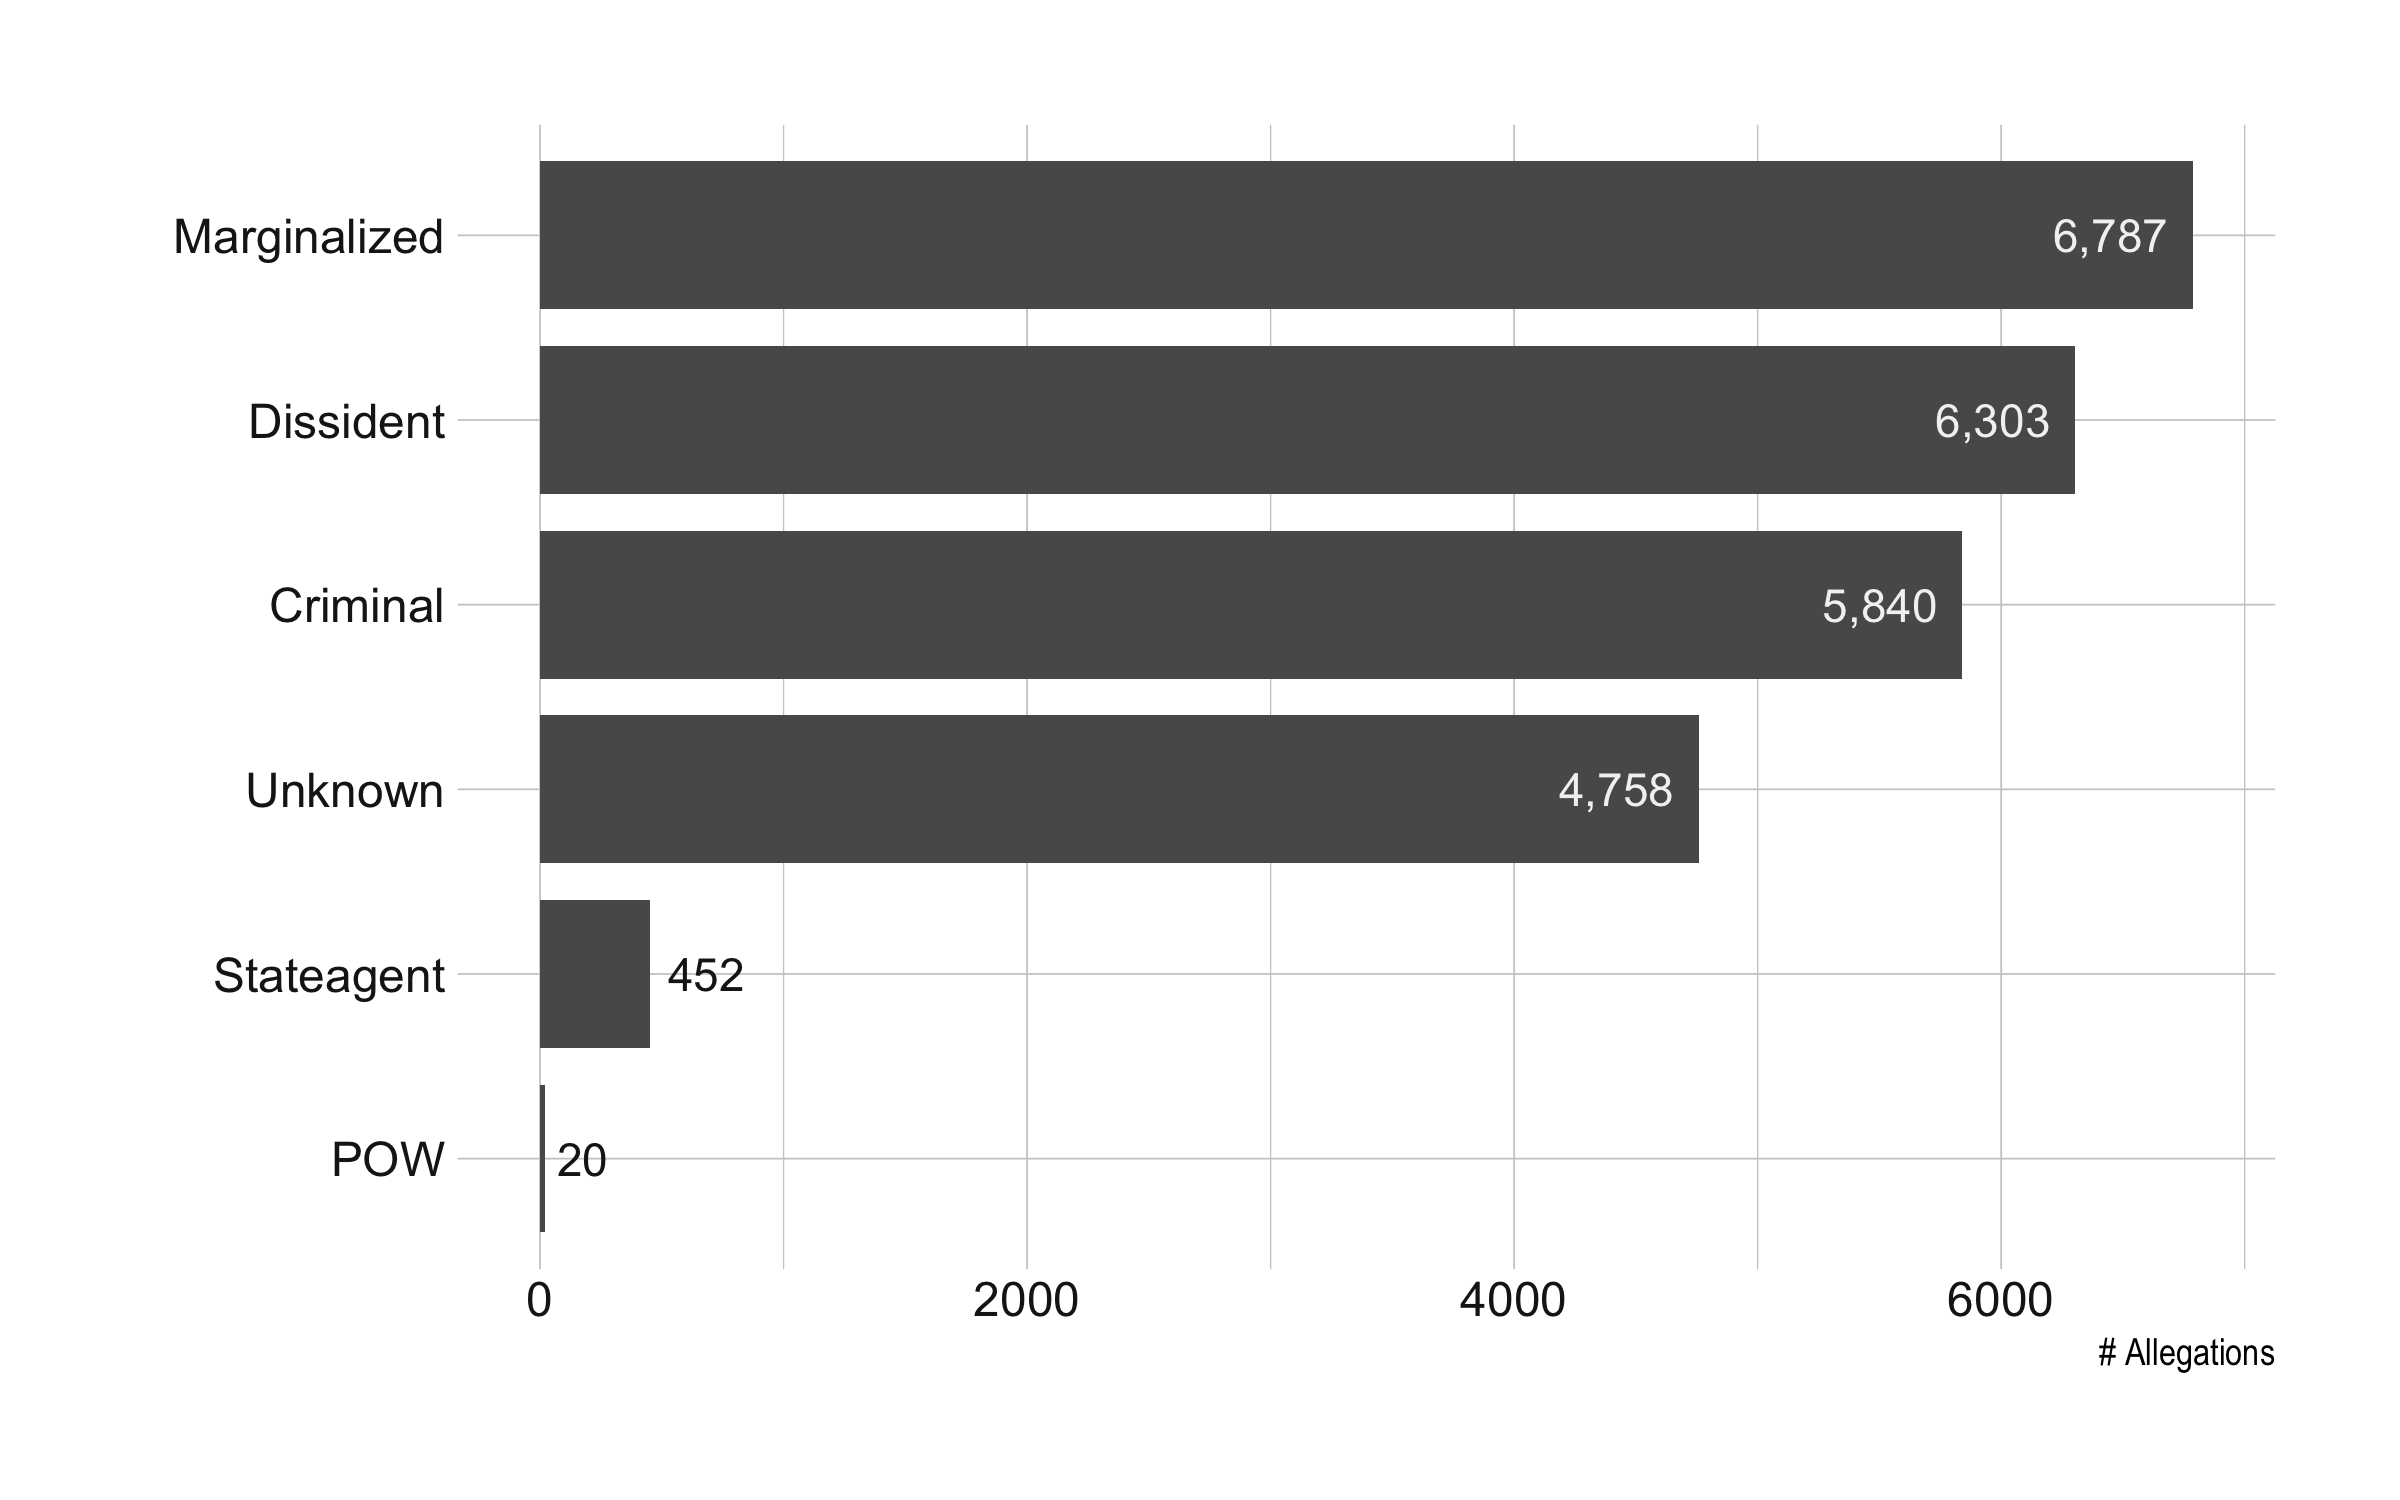
\includegraphics[width=.75\textwidth]{../output/figures/allegations-by-victim.png}
\end{center}
\end{figure}

The ITT specific allegation data suggest that oppressive violence is more common than repressive violence. Figure \ref{fig:victim-types} makes it clear that in most of the allegations in the ITT data the victim is not a dissident. If we include only allegations with a unique, identified victim type, dissidents account for 31\% of allegations, and are the second most common victim type after members of marginalized groups (38.8\%).\footnote{The ITT defines a member of a marginalized social as someone who ``is tortured by the state for the purpose of social control (i.e., humiliation or other punishment to establish that [1] her/his behavior was inappropriate and [2] that the state can abuse her/him with impunity), rather than for the collection of information.'' It lists as candidates immigrants, asylum seekers, the homeless, geeks, punks, skinheads, as well as minorities, e.g., sexual and national (ITT Codebook, p.\ 25--26).} Criminals account for 27.7\% of these allegations, while POWs and state agents combined account for less than 3\%. If we add to our count of dissident allegations cases where the victim falls into the dissident category and at least one other category, then allegations involving the torture of dissidents make up about 38\% of all of the events in ITT with an identified victim type. Of all of the instances of torture publicized by AI between 1995-2005 where the identify of the victim was mentioned, the victim was not a dissident about 62\% of the time.\footnote{See \citet[][pp.\ 3-4]{Haschke2018}, who reports that allegations where the victims are dissidents make up a minority of all allegations even in autocratic countries.} 

The ITT data do not constitute a census of cases of torture. Its creators encourage users to treat the data as what they are, {\em allegations} of torture, rather than a count of cases of torture.\footnote{See \citet{HillMooreMukherjee2013} for an analysis of the CIRI torture scale that suggests AI produces credible information about torture. See also \citet{ConradHillMoore2018}, who analyze ITT using a model that accounts for the fact that allegations represent a subset of all cases of torture.} It should be noted that, as a measure of actual torture, the the ITT data are at least as valid as existing torture scales, which are created partly, and in some cases entirely, from the same set of documents, but record less information about the abuse described in those documents. With this in mind, an examination of the allegations themselves can be instructive for our immediate purpose, which is simply to show that state violence extends well beyond the abuse of dissidents. Taking ITT as an indication, it is plausible that oppressive violence is at least as common as repressive violence. 
%This means that explanations for state violence that focus on the repression of dissent leave many, perhaps most, cases of violence unexplained. 

%Despite the fact that perpetrators of oppressive and repressive violence have distinct motives, it is possible that these kinds of state violence tend to occur in similar social, political, and economic contexts and so will be predicted by many of the same factors. If this were the case it may not be consequential to use measures that aggregate the two, as is common practice. Of course, we cannot know whether this is the case unless we disaggregate the two and consider them separately. 
Additionally, the ITT data suggest that the torture of different victims follow quite different patterns. Figure \ref{fig:correlation-matrix} shows the correlations between allegation counts for the four most common victim types. Each plot displays the across-country average correlation coefficient for that pair of victim types, labeled $\bar{r}$. These correlations, if we exclude the self-correlations on the diagonal, are fairly close to the global average of .34. So it is not the case that countries that torture dissidents are especially prone to torture marginalized groups and criminals as well. This disconnect is even more pronounced at the country level. In each plot off of the diagonal, the gray histogram in the background shows the distribution of within-country correlation coefficients for that pair of victim types. About 20\% of the within-country correlations are 0 or negative, i.e.\ increases in allegations of torture related to one kind of victim are associated with {\em decreases} in allegations of torturing another kind of victim. The general point is that allegations of torturing different kinds of victims are only loosely related. In other words, those countries that (allegedly) torture dissidents  do not necessarily (allegedly) torture criminal suspects or marginalized individuals. 

\begin{figure}
\begin{center}
\caption{}
\label{fig:correlation-matrix}
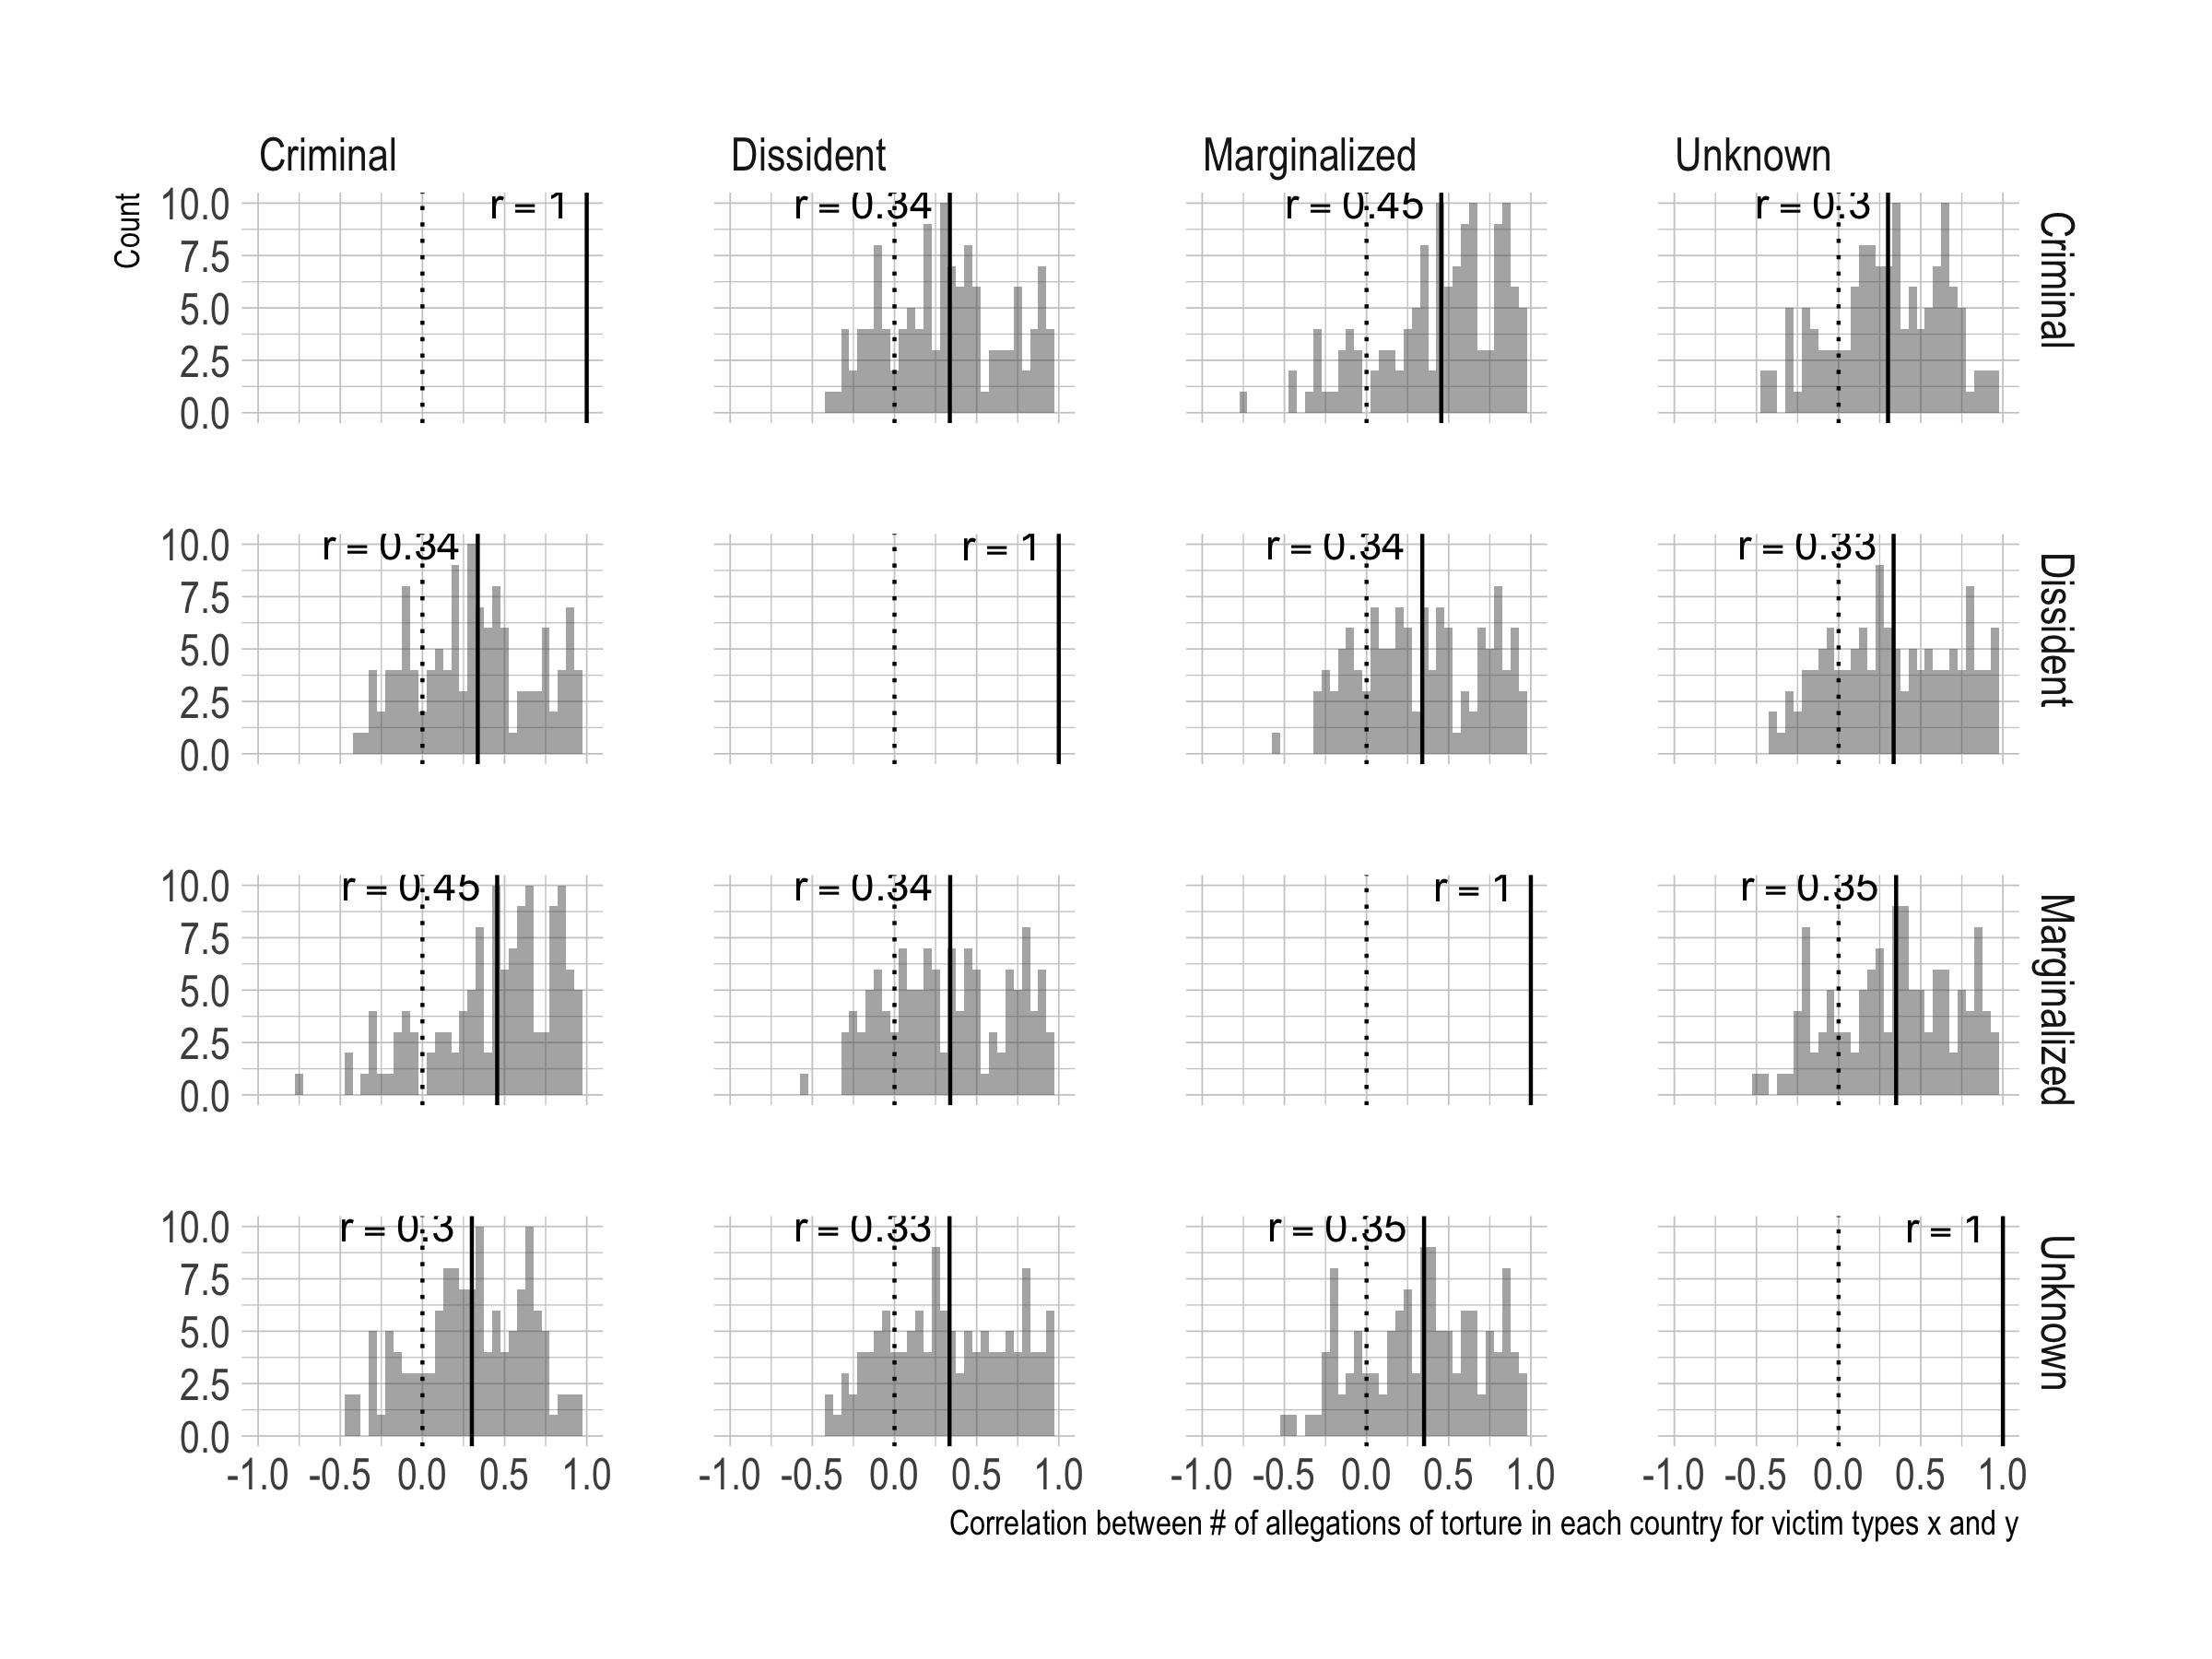
\includegraphics[width=.99\textwidth]{../output/figures/allegations-by-victim-pairwise-correlations.png}
\end{center}
\end{figure}

\section*{Analysis}

The ITT data cover the years 1995 to 2005, 11 years in total. Our data consist of country-years for independent states during that period, following the Gleditsch and Ward list \citep{gleditsch:ward:1999}. This makes for a total of around 1,600 observations. In the raw allegation data, a single allegation may specify any number of six different victim types. We split events with more than one victim type into separate allegations for each victim type. We then count allegations by country-year-victim type. As discussed above, there are few allegations of torture of POWs and state agents, so we leave these out. We also drop the unstated category from the models below. We analyze separately allegation counts for dissidents, criminals, and marginalized groups, which are the three most common victim types. 

Our analysis uses as covariates measures of electoral competition, institutional constraints on the executive, legal barriers to state-imposed detention, and social hierarchy. Electoral accountability and constraints on the executive are the political institutions that receive the most focus in the literature on state violence \citep[e.g.,][]{Davenport2007}. Previous analyses that use victim-specific indicators in ITT fail to find a clear relationship between these institutions and violence against criminals and marginalized individuals \citep{Haschke2018,JacksonHillHall2018}. These studies both use the ITT ``level of torture'' scale from the country-year version of ITT \citep{conrad2013disaggregating} rather than the specific allegations data. We use a binary measure of electoral competition from \citet{cheibub2010democracy}, which is used in \citet{Haschke2018} and \citet{JacksonHillHall2018}. This makes our results comparable to previous studies. This indicator also has the advantage of being based on an operational definition of competition that is less likely to overlap with repressive violence than those used by other measures of competition \citep[See][]{Hill2016}. We take two measures of constraints on the executive from the Varieties of Democracy data (V-Dem) \citep{Vdem}. One captures judicial constraints, and is created from component scales that measures judicial independence and executive compliance with the judiciary. The other indicates the extent to which the legislature exercises effective oversight of the executive. 

For legal barriers to detention we use several indicators from the Comparative Constitutions Project \citep{CCP2014}. From these data we take several binary indicators of specific constitutional provisions, which are all coded one if the relevant provision appears in the national constitution. One of these indicates the inclusion of an explicit reference to due process rights. Another is coded one if the constitution contains a provision for {\em habeas corpus}, or protection from unjustified detention. This encompasses provisions that prohibit arbitrary detention, create a requirement of formal accusation, or arrest based on a warrant or court order. We also include a measure of whether the constitution includes a provision allowing for the possibility of pretrial release. Such provisions include those that ban the imposition of excessive bail, or state that bail cannot be refused or denied without just cause. Another indicator measures whether there is mention of the right to a fast trial, or a trial within a reasonable time. 
%Finally, we include a measure of explicit constitutional bans on torture. 

To measure social hierarchies we rely on two data sources. One is the Ethnic Power Relations data (EPR), from which we take a measure of the proportion of a country's population that belongs to an identifiable ethnic group that is excluded from national politics, as well as a count of the number of excluded groups  \citep{vogt2015integrating}. ``Excluded'' means the group is either not represented in the executive branch, is actively discriminated against in public politics, or is concentrated in a region that is (possibly {\em de facto}) autonomous from the central government.  The other source we use is the V-Dem data, from which we take four measures. Two indicate the extent to which political power and influence are distributed evenly across social groups. The first of these considers whether groups defined by class (disparities in wealth) have differential influence. The second considers whether groups defined by ethnicity, language, religion, race, region, or caste have equal unequal influence. The other two indicators measure whether different class or ethnic groups enjoy the same civil liberties protections, where civil liberties are defined to include access to justice, property rights, freedom of movement, and freedom from forced labor. 

Our regression models are all Poisson models with random intercepts for countries. We include random intercepts 
%for two reasons. The first is that we will evaluate our models in part by their ability to predict outcomes, i.e. model fit, and including random country intercepts improves model fit a lot. 
because, by soaking up between country variation in outcomes with the intercepts, we can be more certain that any associations we find for variables of interest are not spurious correlations driven by other differences between countries. The downside is that, to the extent that the factors we examine (some of which do not vary much across time) really do account for cross-country differences in torture allegations, we are stacking the odds against finding so. 
%The number of observations per group are not very large, 11 years per country at most, which could be problematic both for estimating model parameters and overfitting. The former seems to be more of an issue than the latter, as out of sample accuracy is fairly close to in-sample accuracy. And to the extent that things, some of which don't vary much across time, really do account for cross-country differences in torture allegation levels, we are stacking the odds against finding so. 
We begin by estimating a baseline model that includes (the natural logs of) GDP per capita and population size,\footnote{Both of these are taken from the World Development Indicators.} INGO restricted access from the ITT data, per the codebook \citep[][p.\ 17]{ITTsaguide}, and a measure of internal conflict resulting in at least 1,000 battle deaths from the UCDP armed conflict data \citep{Themner2014}. We then evaluate the relationships between our variables of interest and the three allegation counts in separate models, where each model includes the variable of interest plus the controls. 

\begin{figure}
\begin{center}
\caption{Coefficient estimates for Poisson regression models of torture allegation counts by victim type. All models include random country intercepts.}
\label{fig:coefs}
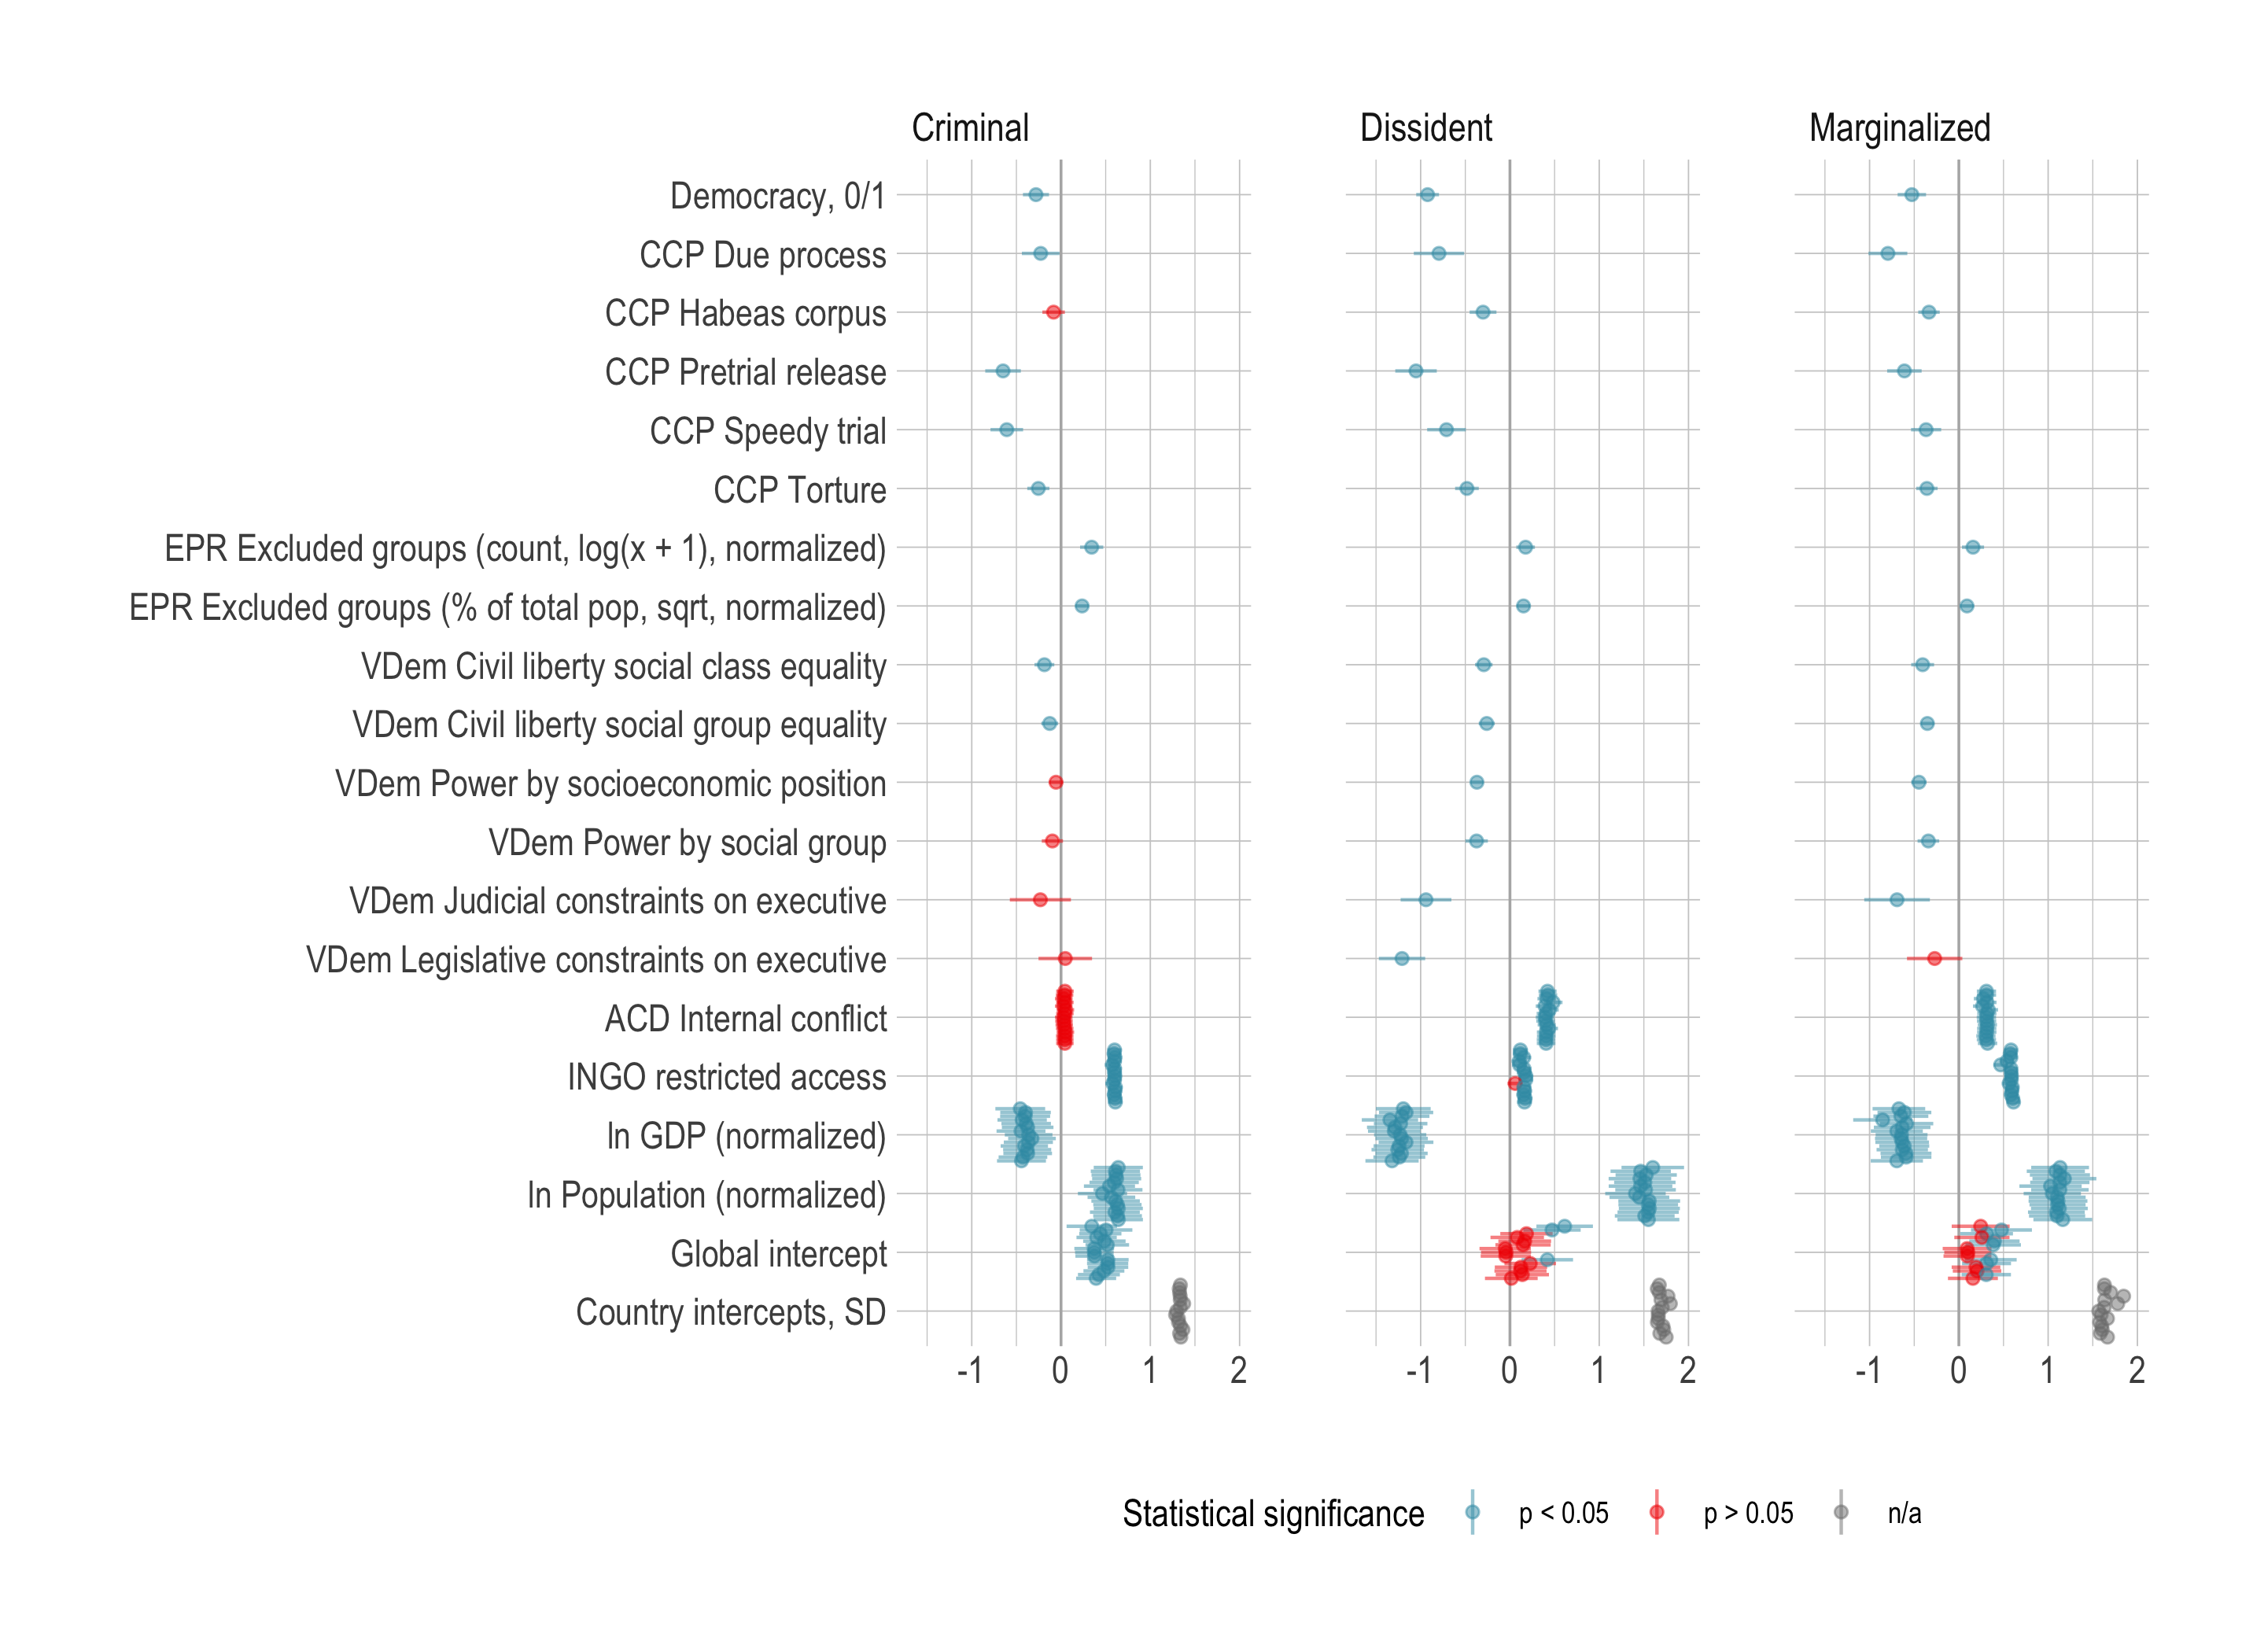
\includegraphics[width=.99\textwidth]{../output/figures/core-models-coefplot.png}
\end{center}
\end{figure}

Figure \ref{fig:coefs} displays the coefficient estimates from all models with 95\% confidence intervals, as well as the global intercepts and the standard deviations of the random intercepts. For control variables, which are included in all models, multiple estimates are displayed. We note first that the coefficients for the binary democracy measure are all negative and statistically significant. The estimate for the dissident model is largest, followed by marginalized individuals and then criminal suspects. This ordering is consistent with our expectation that electoral competition is more strongly associated with repressive than oppressive violence. However, this result contradicts previous findings, which suggest that democracy has no discernible relationship with the torture of marginalized groups, and only a weak relationship with the torture of criminal suspects \citep{Haschke2018,JacksonHillHall2018}.  

The coefficients from the models that include constitutional provisions to curb arbitrary or lengthy detention are all negative, and significant in all but one case, indicating that, in general, these provisions are negatively related to allegations of torture. The only exceptions is the coefficient for {\em habeas corpus} in the models using the criminal suspects victim type. The estimates are similar across victim types. This is perhaps not surprising since rules about discretion over detention should apply to anyone in the state's custody, though we would expect some of these to be more relevant to criminal suspects than other kinds of victims.      

The estimates for excluded population from the EPR data are all positive, which is expected. Surprisingly, however, the estimate is largest for criminal suspects. 

The V-Dem indicators of social hierarchy all have the expected sign, though two estimates are insignificant: the variables measuring the extent to which political power is shared equally across class and ethnic groups are insignificant in the models for criminal suspects. Other than this the estimates are similar across models, though they are slightly larger (in absolute value) for the marginalized individual models.   

Turning to the measures of executive constraints from V-Dem, estimates for judicial constraints are all negative. For criminal suspects the coefficient is not significant. The estimate for marginalized individuals is significant, however, which contradicts the finding reported in \citet{JacksonHillHall2018}. This in combination with the result for electoral competition suggests that there are some differences between the ITT country-year data and the specific allegations data that may be worth exploring. For legislative constraints the coefficients are negative for dissidents and marginalized individuals, but insignificant for the latter. The estimate for criminal suspects is slightly positive and insignificant. 

The estimates for the control variables are generally in line with previous findings. Notably, GDP per capita is more strongly associated with allegations of torturing dissidents than with allegations related to the other victim types. The estimates for armed conflict are largest in the case of dissidents and marginalized individuals, and are insignificant for criminal suspects. 

In addition to count regression models, we evaluate the predictive power of each covariate. While statistical significance is a useful criterion for evaluating model results, statistically significant coefficients do not necessarily translate into increased predictive accuracy \citep{ward2010perils,HillJones2014}. For this purpose we use a machine learning predictive model called XGBoost. The model is an ensemble of decision trees, where each decision tree is specifically trained to reduce leftover prediction error given the current ensemble prediction. Each component decision tree itself is a very simple model that predicts allegation counts by splitting the input data into several groups using cut-points for selected independent variables that are chosen to minimize variation in the outcome within the groups. The model determines the importance of a particular input variable in predicting the outcome by calculating the reduction in prediction error that results from including that variable in the model. 

Variable importance scores for each variable are displayed in Figure \ref{var-imp}. For each variable the figure shows an importance score for each victim type. Across victim types, the set of variables that add the most predictive accuracy is very similar, though the orderings are slightly different. GDP per capita, population, legislative constraints, and judicial constraints all contribute to relatively large improvements in prediction. For all victim types, GDP per capita outperforms every other variable. Population is second for criminal suspects and marginalized groups, while legislative constraints is second for dissidents. For allegations involving marginalized individuals, the number of excluded ethnic groups is third, followed by legislative constraints. For dissidents, population and judicial constraints are third and fourth respectively, followed by the variables that measure ethnic exclusion. For criminal suspects, legislative constraints is third, followed by judicial constraints and then by the V-Dem variable that measures equality in power/influence across socioeconomic groups. Notably, only for the marginalized victim category does ethnic exclusion outperform either of the executive constraints variables. The binary democracy indicator and constitutional provisions variables (also binary) add little predictive power, though we add that decision trees favor variables that can take on many values over those that can take on few. 

Though this set of variables does relatively well at predicting allegations for each victim type, the importance scores for individual variables vary quite a bit across victim types. Notably, legislative and judicial constraints are better at predicting the outcome for dissident victims than for the other two victim types. 
%This is likely due to the fact that our regression models include random intercepts for countries, which account for much of the across-country variation in allegations. Coefficient estimates in those models are based partly on within-country variation. Variables that do well at accounting for across-country variation but not within-country variation will likely have small coefficient estimates. In contrast, the XGBoost results are likely picking up on the ability of the variables to predict the outcomes across countries, as most of the variation in allegation counts is across rather than within countries.  

\begin{figure}
\begin{center}
\caption{XGBoost variable importance for predictive accuracy.}
\label{var-imp}
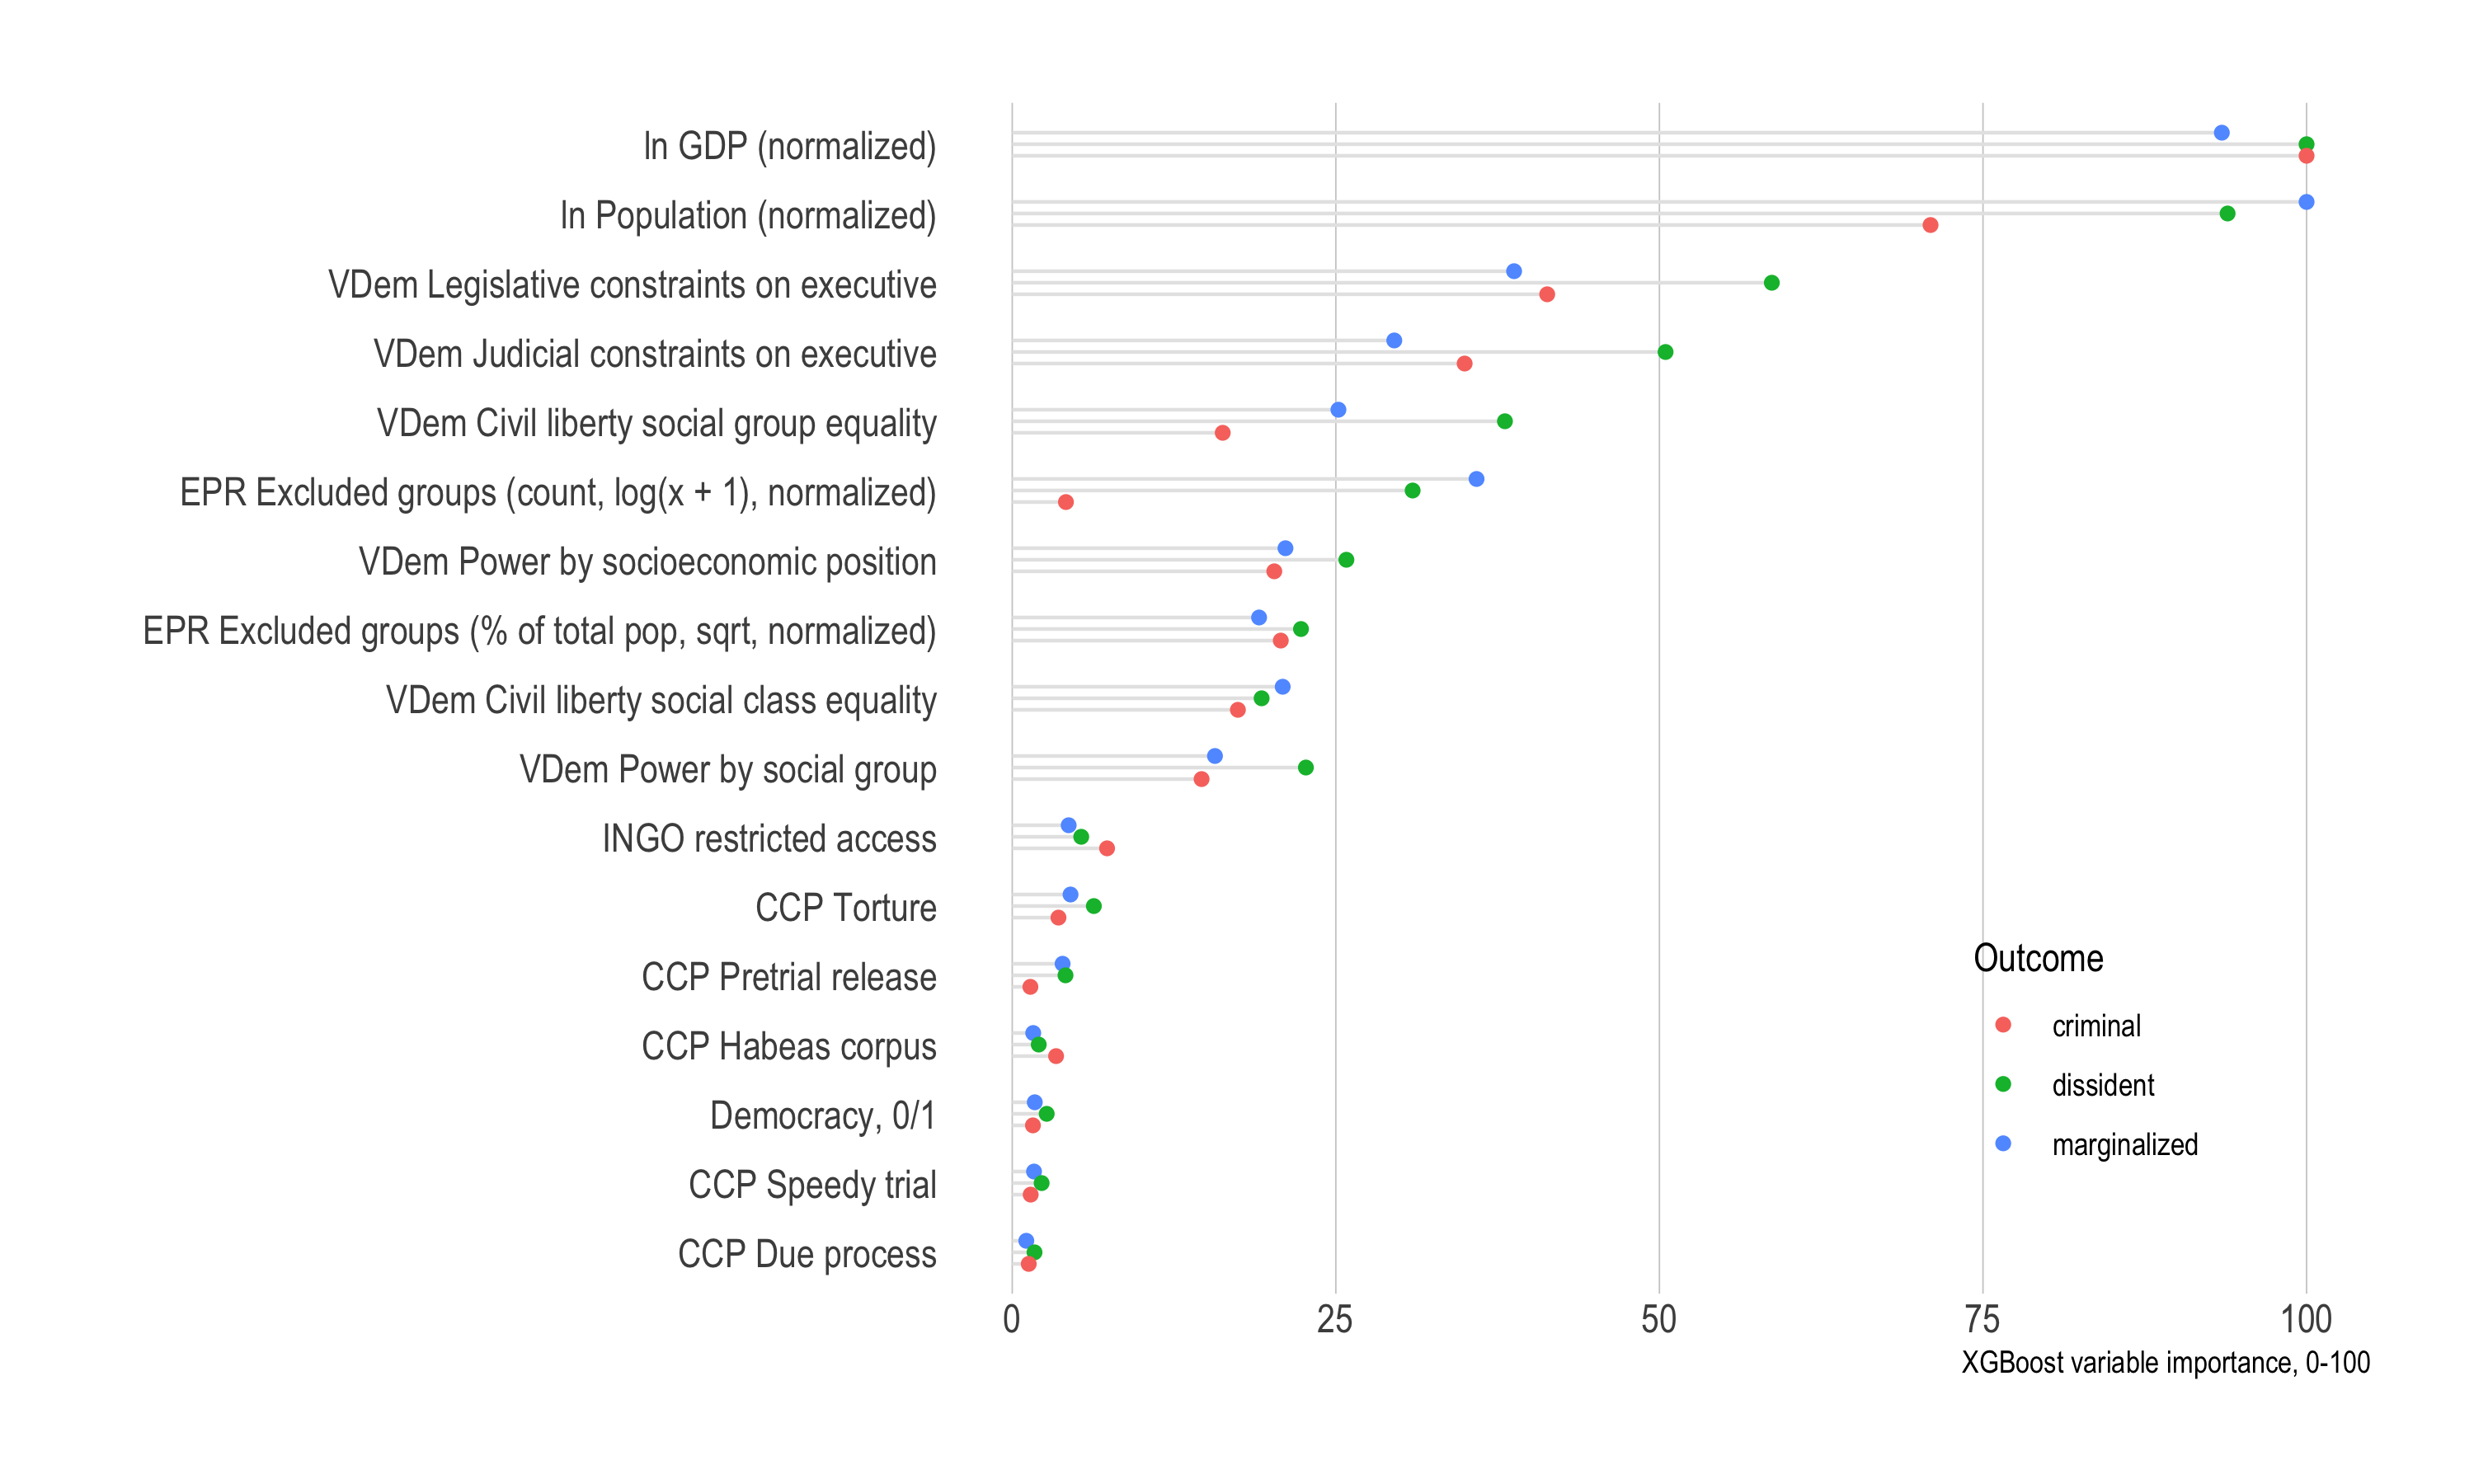
\includegraphics[width=.99\textwidth]{../output/figures/xgboost-variable-importance-v1.png}
\end{center}
\end{figure}

%In addition to the coefficient estimates for the variables that interest us, we also consider the impact of adding a variable on model fit, and out of sample fit specifically. This indicates how well any empirical results are to generalize outside the 11-year coverage of the data. To derive out of sample predictiosn we used 11-fold cross-validation, which roughly corresponds to predicting one year of outcomes with the remaining 10 years of data. 

%The last model is a commonly used machine learning predictive model, XGBoost, which provides another benchmark of the levels of prediction accuracy one should expect to be feasible. Hyperparameters for this kind of model are usually tuned via cross-validation. In order to be able to compare the cross-validation predictions to those from the count models, we did not do this and instead left hyperparameters at their default values.

Finally, Figure \ref{oos-fit} summarizes the out-of-sample fit for the XGBoost and regression models. These were obtained using 11-fold cross-validation, and the figure shows continuous rank probability scores (CRPS), mean absolute error (MAE), and root mean squared error (RMSE); for all measures lower values mean better model fit. The best-performing regression model for each combination of outcome and fit statistic is labeled in the plot. Some variables that did not fare well in the XGBoost analysis do improve out-of-sample fit in the regression models, most notably the binary democracy variable (for dissidents) and the CCP speedy trial variable (for criminal suspects). In general, the variables of interest typically increase fit compared to a random effects-only control model. It is also notable that the XGBoost model outperforms the regression models by a large margin except for marginalized groups, where it only slightly outperforms the model that includes V-Dem's power by socioeconomic position (based on RMSE). 

\begin{figure}
\begin{center}
\caption{Out-of-sample fit.}
\label{oos-fit}
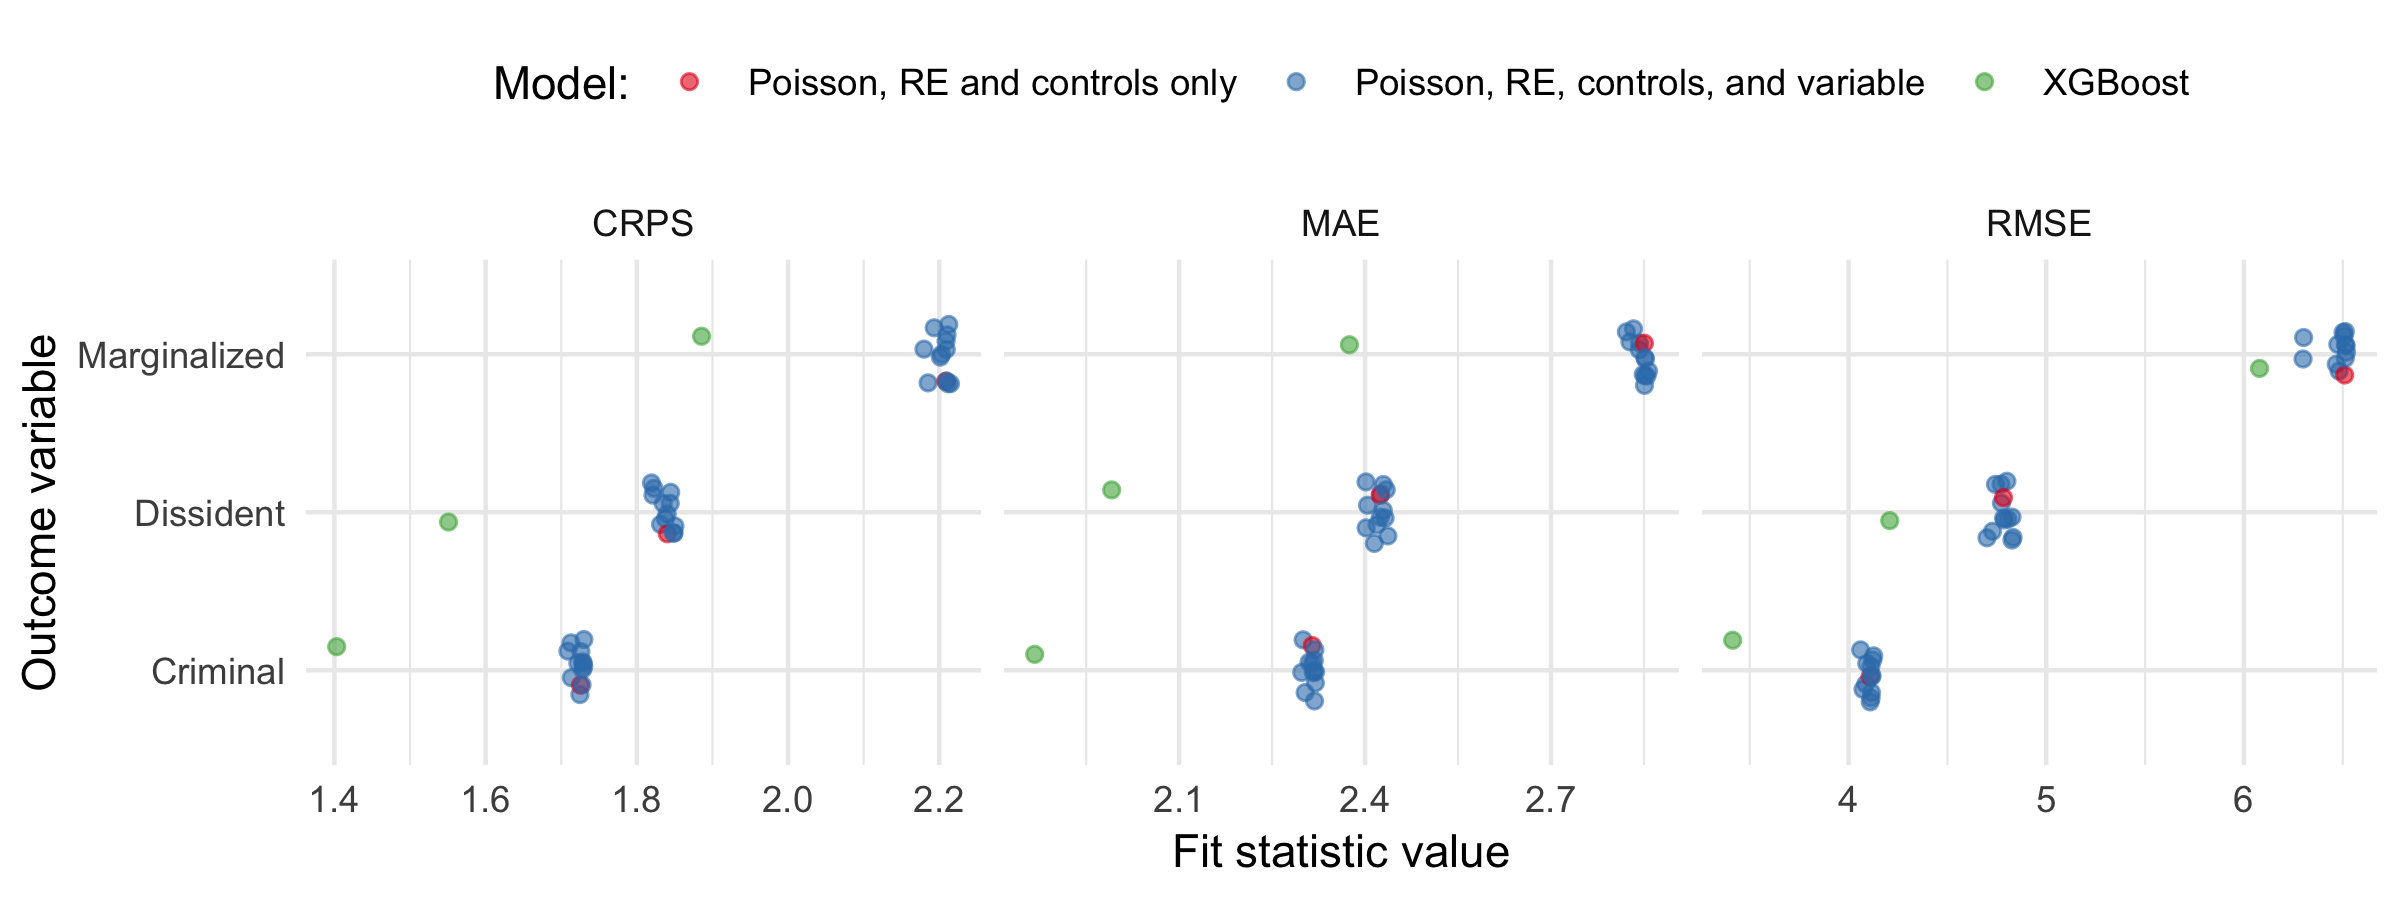
\includegraphics[width=.99\textwidth]{../output/figures/oos-fit-all.png}
\end{center}
\end{figure}

\section*{Conclusion}

Based on our analysis, we draw three broad conclusions about the differences between repressive and oppressive violence. First, the political institutions that receive the most attention in the literature, electoral competition and executive constraints, appear to be better at protecting dissidents from physical abuse than other kinds of victims. That is, they are more reliably associated with repressive violence than oppressive violence. On the one hand, some political institutions are associated with oppressive violence in our analysis. Competitive elections are related to allegations involving all the victim types we examined, including those that we take as indicators of oppression. Judicial constraints are related to allegations of torturing marginalized individuals. Legislative and judicial constraints also predict allegations of oppressive violence well relative to most of the factors expected to influence oppression. On the other hand, these institutions, in particular competition and legislative constraints, are more strongly associated with repressive violence than oppressive violence. They are also much better at predicting repressive violence than oppressive violence. This supports the claim that explanations for state violence that focus on political institutions are better suited to explaining repressive violence. 

Second, the conditions we identify as important influences on oppressive violence have some explanatory and predictive power, though perhaps less than expected. The most promising result on this count is that ethnic inclusion is negatively associated with violence against marginalized individuals and especially criminal suspects in our regression models, and predicts violence against marginalized groups better than judicial constraints. Constitutional provisions related to detention are associated with oppressive and repressive violence, and in one case has reasonable predictive power for abuse of criminal suspects. We add that we use these provisions only as proxy measures for oversight and monitoring of state-imposed detention. More direct measures of that concept, though difficult to come by, should be useful for future research.     

Finally, we note that the decision to examine different kinds of state violence separately should be guided by the explanation for violence one wishes to test. Because most existing explanations have in mind repressive violence, it is not appropriate to examine oppressive violence to determine if they are incorrect. However, some arguments are more general. The principal-agent framework discussed above, for example, suggests that allocating resources to monitoring coercive agents, and punishing those responsible for abuse, should reduce both oppressive and repressive violence.   

%On the other hand, democracy. We've explained why it has to be related to abuse of dissidents. But take case where operational definition doesn't overlap w/ repression. E.g., legislative constraints. When opposition can check executive, abuse of dissidents is less likely. Makes sense that the opposition would oppose abuse of gov't opponents, since they are in a similar position. But not same w/ criminals. In fact, things that matter for other two don't matter for criminals, suggesting this may be most difficult group to protect.   

\clearpage
\begin{singlespace}
\bibliographystyle{apsr}
\bibliography{beg_hil}
\end{singlespace}

\end{document}




